\subsection{Coupled Cluster Doubles with Perturbative Triples and Realistic Potentials}

As a final data set with SRE, we will attempt to predict the converged correlation energies for SNM using the CCD(T) approximation.  The CCD(T) approximation has significantly higher time requirements than the CCD approximation, as we saw with the PNM case.  But this difference in time will be even higher more drastic for SNM since there will be a higher number of single-particle states. Remember that the expected computational time for a CCD calculation is $O(M^6)$, and for a CCD(T) calculation, it is $O(M^7)$.  This extra factor of M can contribute significantly to the run time since it can be as large as M = 2,956 for the fully converged calculations.  However, for this case, due to the high computational costs, we have truncated M to only 23 energy shells or M = 2,060.  At this level, the correlation energies have converged to an order of 10$^{-3}$ or less, so it should be sufficient for this work, but it is important to note that if the calculations were carried all the way out to M = 2,956 then the run times would be much higher.  We can see in Fig. \ref{fig:snm_ccdt_pert_times} that the CCD(T) run times (blue) are, in fact, much higher than the CCD run times.  The CCD(T) data was collected on Oak Ridge National Laboratory's Andes supercomputer using 3.0 GHz and 64 MPI nodes.  Since the CCD and CCD(T) data was collected on different supercomputers and with a different number of MPI nodes, in Fig. \ref{fig:snm_ccdt_pert_times}, we have standardized the run time by reporting it as node hour per GHz.

\begin{figure}
    \centering
    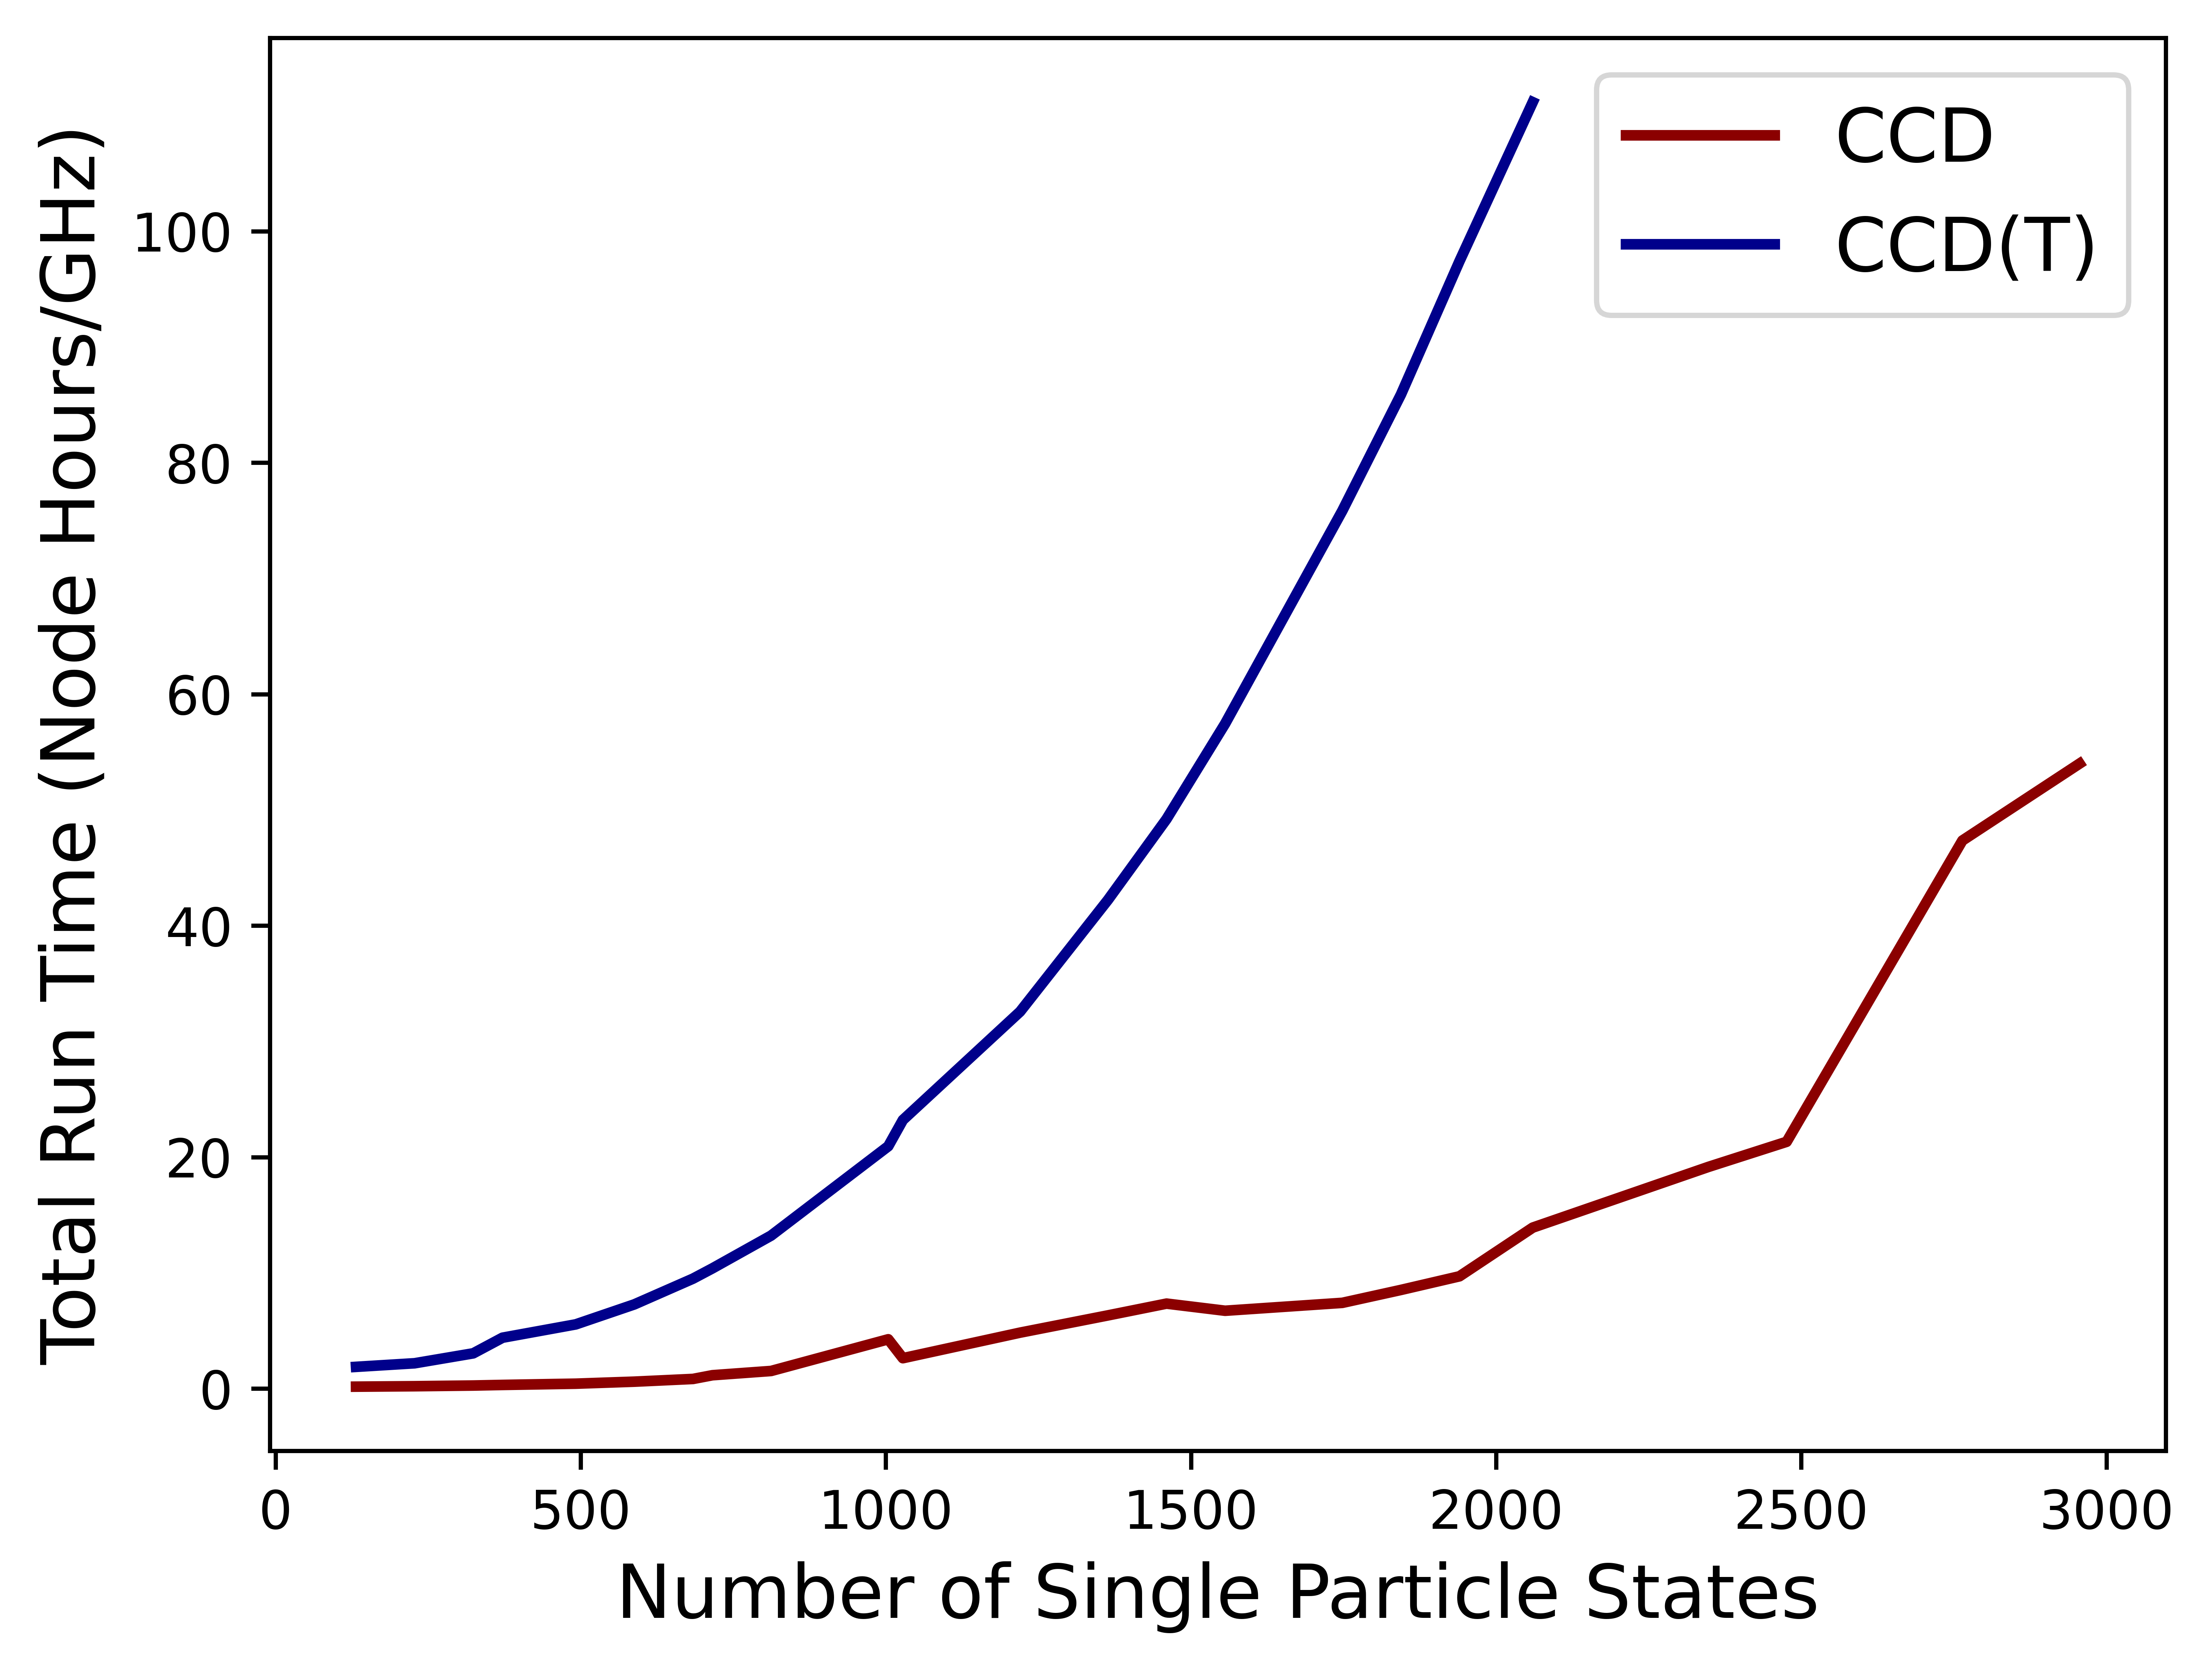
\includegraphics[scale=0.75]{Images/Chapter8/PRX_ORNL1_Fig2b.png}
    \caption{The run times (in node hours per GHz) for CCD calculations of SNM (red) and CCD(T) calculations of SNM (blue).  The CCD calculations were performed on processors which ran at 2.4GHz and used 24 MPI nodes, while the CCD(T) calculations were performed on processors that ran at 3.0GHz and used 64 MPI nodes.}
    \label{fig:snm_ccdt_pert_times}
\end{figure}

The average time to perform a CCD calculation of SNM at M = 2,956 is 84.12 node hours.  However, the average time to complete a CCD(T) calculation of SNM at only M = 2,060 is 335.65 node hours.  However, this significant increase in run time is necessary as the CCD(T) approximation adds some aspects of the $\hat{T}_3$ operator into the calculations neglected in the CCD approximation.  This does make the calculations more accurate (more comparable to an actual SNM system), but we do have to pay the much higher computational cost.  This further motivates the use of the SRE method because here we are taking almost 14 \textit{node days} per density of interest, making studies of, for example, the equation of state of nuclear matter prohibitively expensive.

Fig. \ref{fig:ccdt_pert_sre} shows the results of performing an SRE analysis on CCD(T) calculations of SNM.  The calculations at M = 2,060 are shown with the solid lines, and then SRE predictions are shown with triangular markers, which have error bars that come from the uncertainty of the Gaussian process algorithm; here, we have used six training points (from M = 162 to M = 406), and we have set the SRE sequence length to 1.  This results in an average percent error of 0.65$\%$.  Compared to the average percent error between the data at M = 406 (the largest training point) and the converged energies at M = 2,060 of 14.70$\%$, the SRE method accurately predicts the converged CCD(T) energies from unconverged energies.  Looking at the run times, it takes a total of 2,000.57 node hours to generate the six data points at M = 2,060, but it only takes 721.81 node hours to create the training data needed by the SRE algorithm, which is required to produce these converged correlation energies accurately.  This results in a time savings of 1,278.75 node hours or 53.28 \textit{node days}.

\begin{figure}
    \centering
    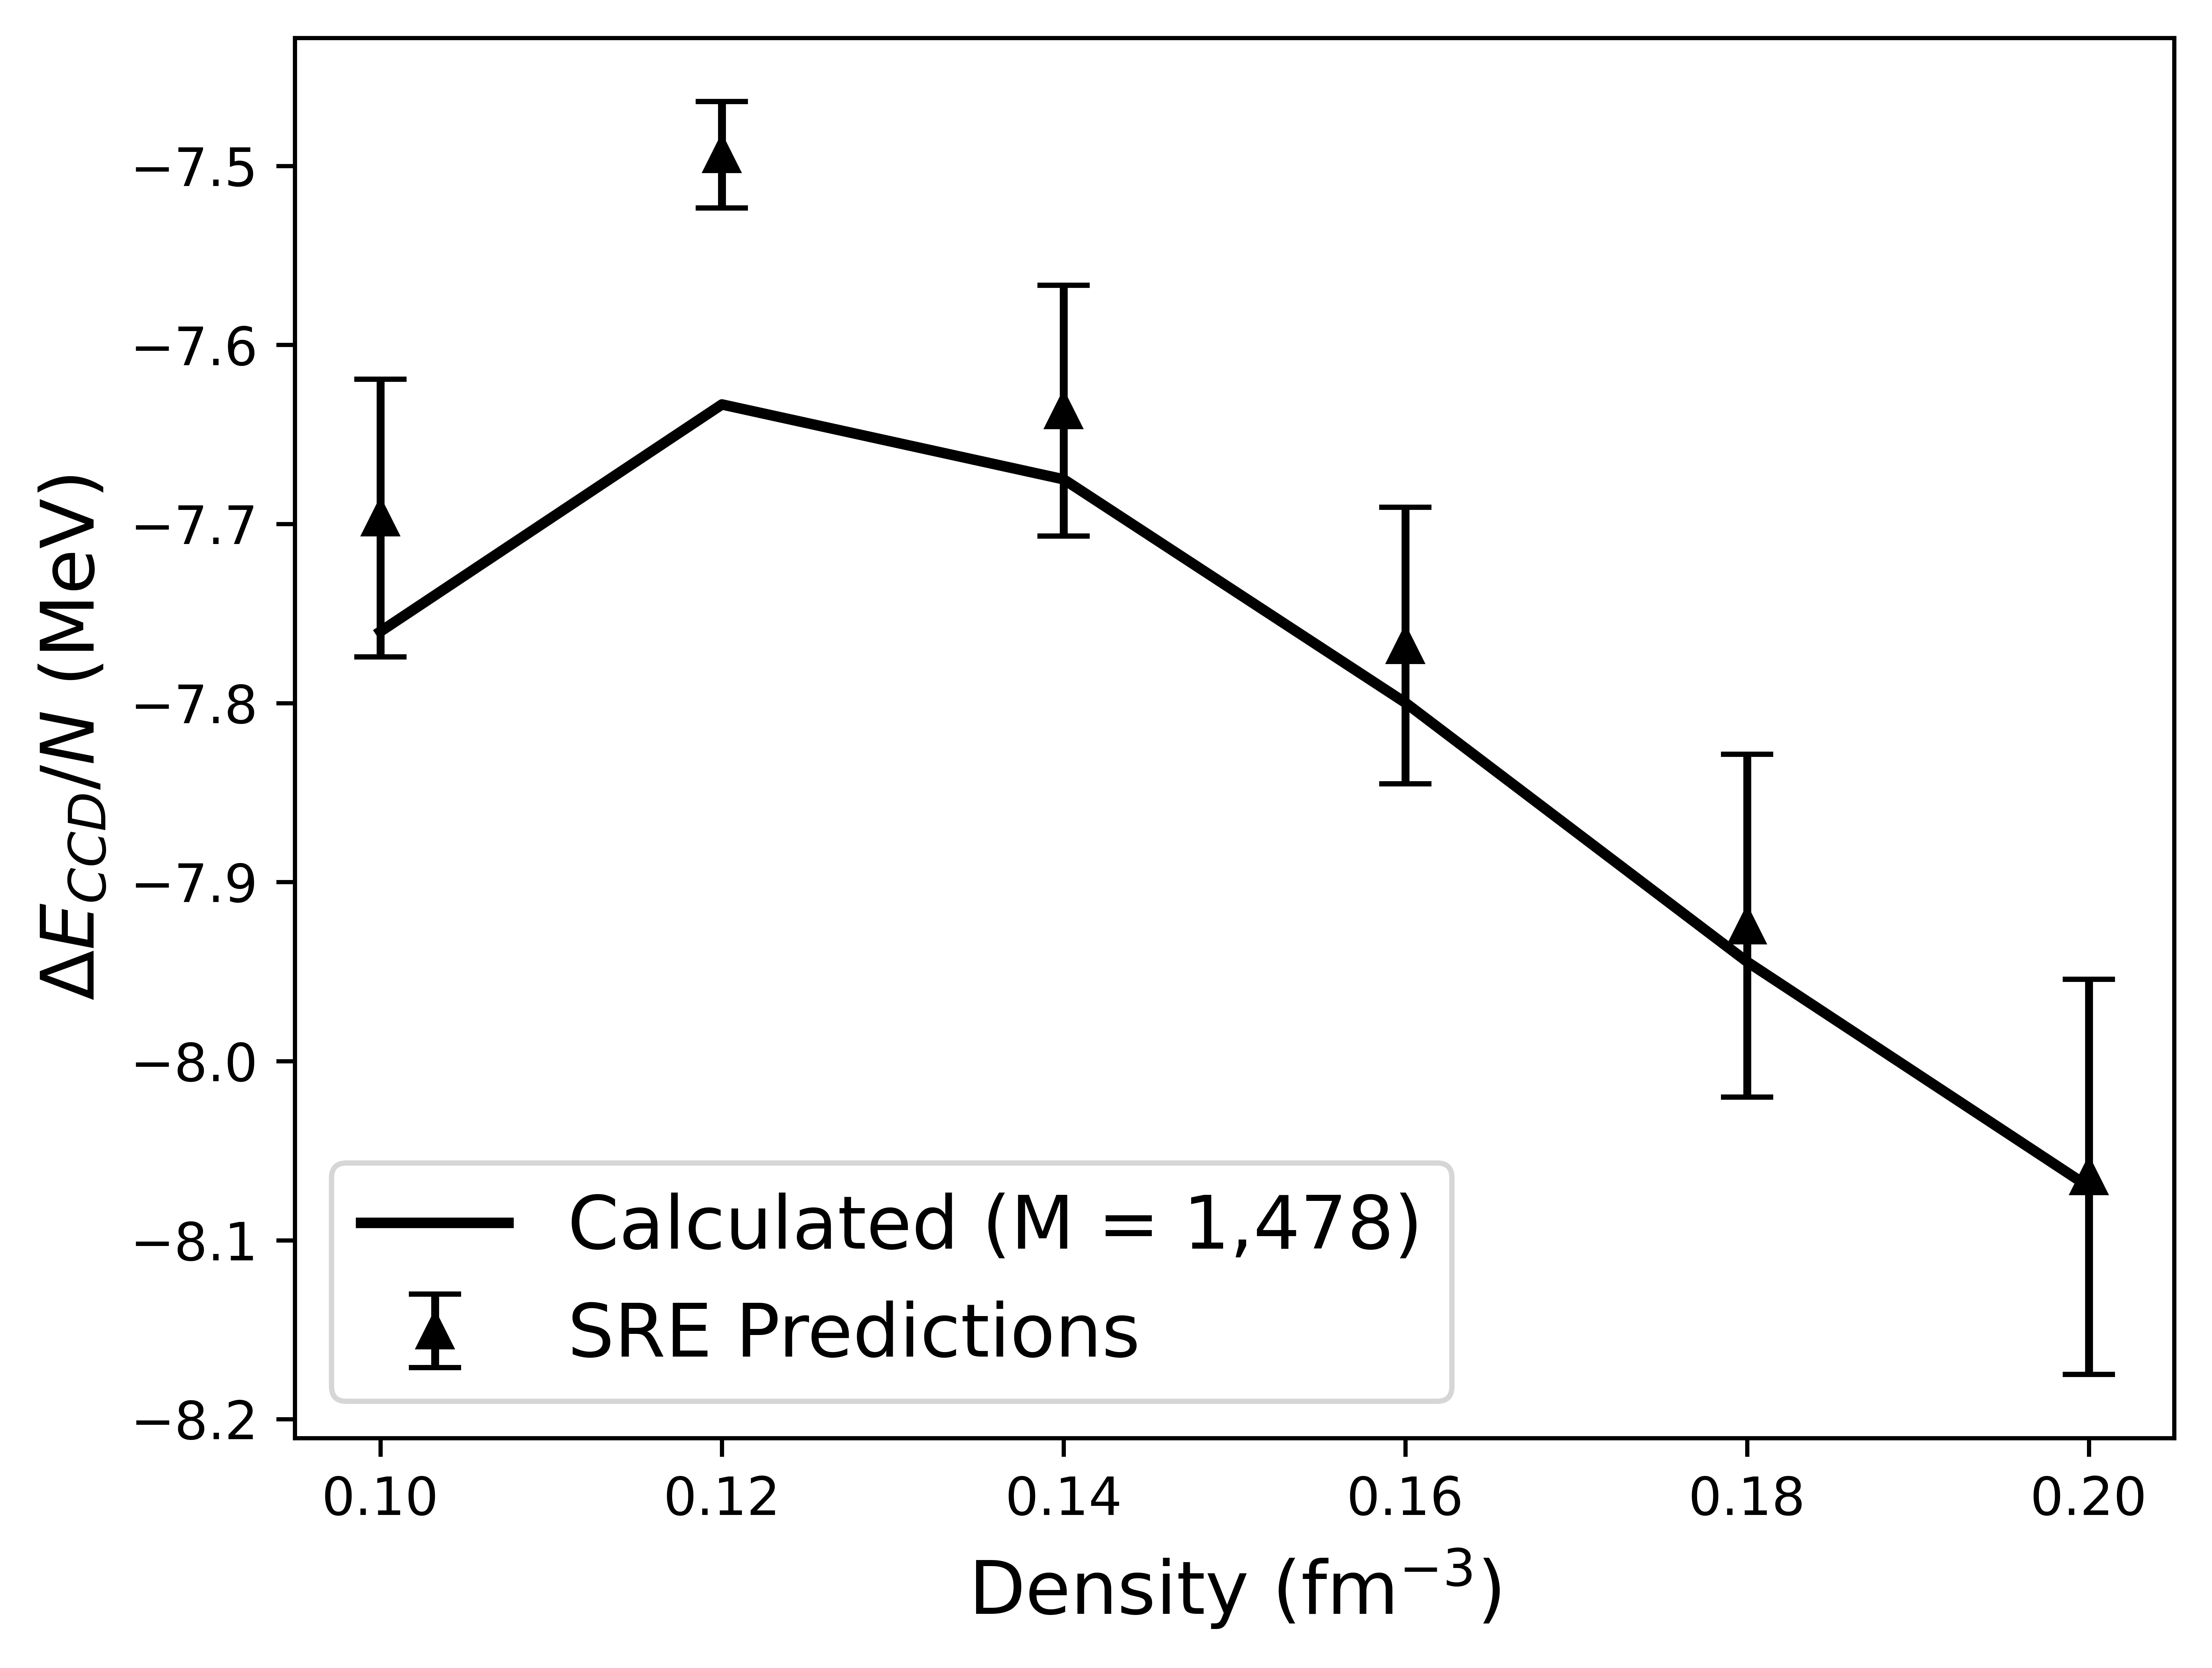
\includegraphics[scale=0.75]{Images/Chapter8/FinalReport4b.png}
    \caption{The CCD(T) correlation energies for SNM calculated at M = 2,060 (solid line) and predicted with SRE (triangular markers).}
    \label{fig:ccdt_pert_sre}
\end{figure}

Finally, we can compare the CCD correlation energies for SNM (red) and the CCD(T) correlation energies for SNM (blue) in Fig. \ref{ccd_ccdt_snm}. The complete calculations at M = 2,956 for CCD and M = 2,060 for CCD(T) are shown with solid lines, and the SRE markers are shown with triangular markers.  We draw two important conclusions from this figure.  First, the CCD and CCD(T) correlation energies are significantly different, so this does justify the higher computational cost of the CCD(T) calculations as the CCD(T) results should more closely model a real system as they take into account some aspects of the $\hat{T}_3$ operator.  Second, we can see that the SRE method performs well on both CCD and CCD(T) data sets, again showing that SRE works well on different coupled cluster data sets with no modifications of the algorithm besides changing the two hyperparameters: the number of training data points and the SRE sequence length.


\begin{figure}
    \centering
    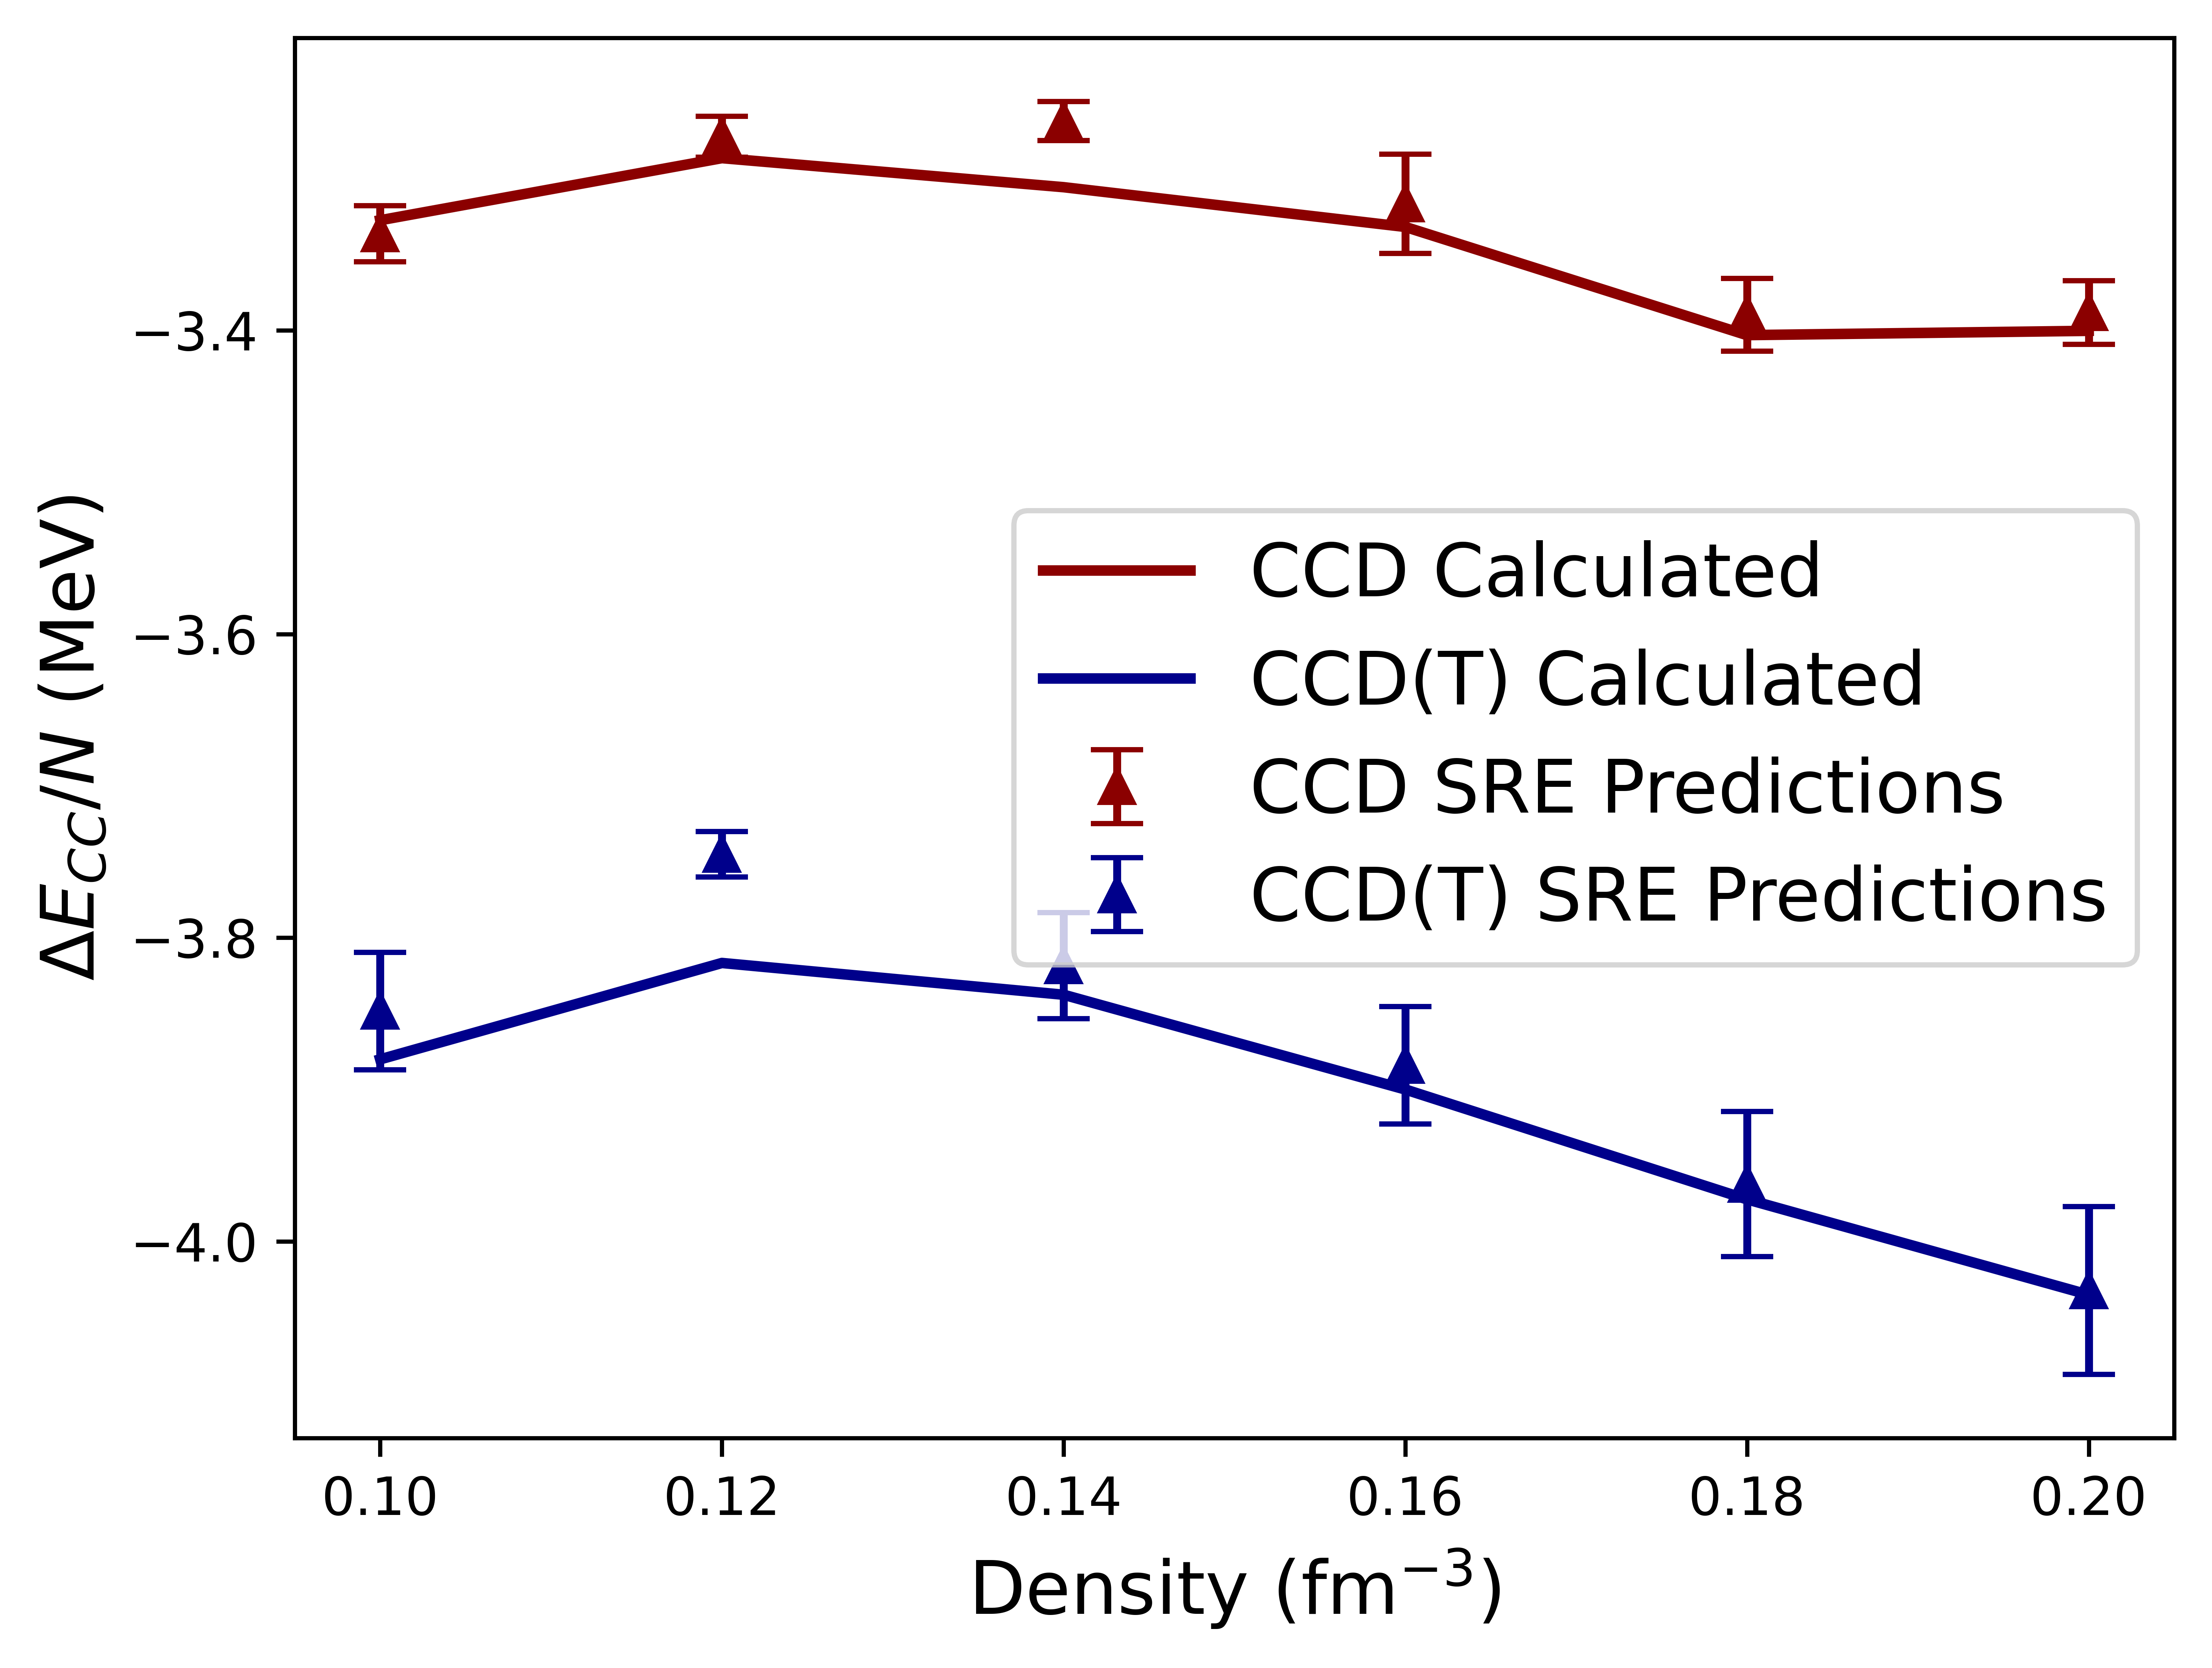
\includegraphics[scale=0.75]{Images/Chapter8/PRX_ORNL1_Fig3b.png}
    \caption{The correlation energies for SNM were calculated with CCD (red) and CCD(T) (blue).  The full calculations at M = 2,956 (CCD) and M = 2,060 (CCD(T)) are shown with solid lines, and the SRE predictions are shown with triangular markers.}
    \label{fig:ccd_ccdt_snm}
\end{figure}